\documentclass{article}
\usepackage{epsfig, latexsym}

\begin{document}

\newcommand{\SOPmin}{${\rm SOP}_{\rm min} \ $}
\newcommand{\POSmin}{${\rm POS}_{\rm min} \ $}
\newcommand{\bs}{\backslash}


\title{
\Huge{CSE 271 -- Fall 2003}\\
\normalsize{Exam 2}\\
\makebox[4in][l]{Name:}
SSN:}
\date{}

\maketitle{}

\begin{tabular}{llll}
\begin{tabular}{c||c}
D & Q+   \\ \hline
0 & 0 \\ \hline
1 & 1 \\
\end{tabular}
&
\begin{tabular}{c||c}
T & Q+   \\ \hline
0 & Q \\ \hline
1 & Q' \\
\end{tabular}
&
\begin{tabular}{c|c||c}
S & R & Q+   \\ \hline
0 & 0 & Q \\ \hline
0 & 1 & 0 \\ \hline
1 & 0 & 1 \\ \hline
1 & 1 & x \\
\end{tabular}
&
\begin{tabular}{c|c||c}
J & K & Q+   \\ \hline
0 & 0 & Q \\ \hline
0 & 1 & 0 \\ \hline
1 & 0 & 1 \\ \hline
1 & 1 & Q' \\
\end{tabular}
\\
\end{tabular}


\begin{enumerate}
\item {\bf (2 pt.)} How many 2:4 decoders are required to construct a 6:64 decoder?
\begin{description}
\item{a) }3
\item{b) }16
\item{c) }21
\item{d) }32
\item{e) }63
\end{description}

\item {\bf (2 pt.)}How many inputs do the AND gates inside a 4:1 mux have?
\begin{description}
\item{a) }2
\item{b) }3
\item{c) }4
\item{d) }5
\item{e) }None of the above.
\end{description}

\item {\bf (2 pt.)} How many data outputs does a 4:1 mux have?
\begin{description}
\item{a) }1
\item{b) }2
\item{c) }4
\item{d) }6
\item{e) }None of the above.
\end{description}

\pagebreak{}
\item {\bf (2 pt.)} If a 16:1 mux is constructed from 2:1 muxes, how
many of the 2:1 muxes get the select line $S_2$?  Note, the select lines
are $S_3, S_2, S_1, S_0$.
\begin{description}
\item{a) } 1
\item{b) } 2
\item{c) } 4
\item{d) } 8
\item{e) } None of the above.
\end{description}

\item {\bf (2 pt.)} If the delay through a single 2:1 mux is 1 unit of time then
what is the propagation delay through a 16:1 mux constructed from 2:1 muxes?
\begin{description}
\item{a) }2
\item{b) }4
\item{c) }8
\item{d) }15
\item{e) }None of the above.
\end{description}


\item {\bf (1 pt.)} How many address bits does a 2kx32 RAM have?
\begin{description}
\item{a) } 5
\item{b) } 11
\item{c) } 21
\item{d) } 31
\item{e) } $2^{32}$
\end{description}

\item {\bf (1 pt.)} How many data bits does a 2kx32 RAM have?
\begin{description}
\item{a) } 5
\item{b) } 11
\item{c) } 21
\item{d) } 32
\item{e) } $2^{32}$
\end{description}

\pagebreak

\item {\bf (2 pt.)} Assuming a word size of 4 bits, interpret 1010 as a 2's complement
number.
\begin{description}
\item{a) }-2
\item{b) }-5 
\item{c) }-6 
\item{d) }-10 
\item{e) }None of the above.
\end{description}

\item {\bf (2 pt.)} Assuming a word size of 4 bits, determine the 2's complement
representation of -3.
\begin{description}
\item{a) }1100
\item{b) }1011
\item{c) }1100 
\item{d) }1101 
\item{e) }None of the above.
\end{description}

\item {\bf (2 pt.)} Assuming a word size of 4 bits and a 2's complement representation,
compute  1101 - 0011
\begin{description}
\item{a) } 0110
\item{b) } 1010
\item{c) } 1000
\item{d) } Invalid answer because overflow occurs.
\item{e) } None of the above.
\end{description}

\item {\bf (2 pt.)} What is $F^+$ for the following circuit when
$A=1$ and $B=1$?
\begin{description}
\item {a) } F
\item {b) } F'
\item {c) } 0
\item {d) } 1
\item {e) } None of the above.
\end{description}

\includegraphics{./Fig2/NANDs}

\pagebreak{}

\item {\bf (3 pt.)} Which statement is realized by the following circuit?

\scalebox{0.7}{\includegraphics{./Fig2/combo}}

\begin{description}
\item{a) } \verb!if (4 > a) then Z = Y+3 else Z = Y+7;!
\item{b) } \verb!if (4 < a) then Z = Y+3 else Z = Y+7;!
\item{c) } \verb!if (4 >= a) then Z = Y+3 else Z = Y+7;!
\item{d) } \verb!if (4 <= a) then Z = Y+3 else Z = Y+7;!
\item{e) } none of the above.
\end{description}

In the following question you are to complete the design of a counter with
the following truth table and circuit diagram.  All that remains is to route
the signals to the mux.  For each of the four questions use the following
letters to code your answer:
\begin{description}
        \item {a)} The output of the ADDER
        \item {b)} 0
        \item {c)} D
        \item {d)} The output of the REGISTER
        \item {e)} None of the above
\end{description}

\begin{tabular}{l|l|l||l}
clk         & $C_1 C_0$ & D & $Q^+$ \\ \hline \hline
0,1,$\downarrow$ & xx   & x & Q     \\ \hline
$\uparrow$     & 00     & x & Q     \\  \hline
$\uparrow$     & 01     & x & 0     \\  \hline
$\uparrow$     & 10     & x & Q+1 mod 16  \\  \hline
$\uparrow$     & 11     & D & D     \\
\end{tabular}

\scalebox{0.65}{\includegraphics[-120mm,0mm][0mm,0mm]{./Fig2/counter.eps}}

\item{\bf (1 pt.)} Which signal goes into the $y_0$ input of the mux?
\item{\bf (1 pt.)} Which signal goes into the $y_1$ input of the mux?
\item{\bf (1 pt.)} Which signal goes into the $y_2$ input of the mux?
\item{\bf (1 pt.)} Which signal goes into the $y_3$ input of the mux?

\pagebreak{}

\underline{For questions 17-20 use the circuit and timing diagram
show below}

\scalebox{0.7}{\includegraphics{./Fig2/ExTim}}

\item {\bf (1 pt.)} What is the value of $Q_1$ at time=25nS?
\begin{description}
\item{a) }0 
\item{b) }1 
\item{c) }Toggling rapidly. 
\item{d) }Input(s) is (was) changed too close to the clock edge to tell.
\end{description}

\item {\bf (1 pt.)} What is the value of $Q_1$ at time=55nS?
\begin{description}
\item{a) }0 
\item{b) }1 
\item{c) }Toggling rapidly. 
\item{d) }Input(s) is (was) changed too close to the clock edge to tell.
\end{description}

\item {\bf (1 pt.)} What is the value of $Q_2$ at time=25nS?
\begin{description}
\item{a) }0 
\item{b) }1 
\item{c) }Toggling rapidly. 
\item{d) }Input(s) is (was) changed too close to the clock edge to tell.
\end{description}

\item {\bf (1 pt.)} What is the value of $Q_2$ at time=39nS?
\begin{description}
\item{a) }0 
\item{b) }1 
\item{c) }Toggling rapidly. 
\item{d) }Input(s) is (was) changed too close to the clock edge to tell.
\end{description}

\pagebreak{}
\item {\bf (4 pt.)}The counter shown in the figure below operates according to
truth table given.  Determine the count sequence on the
$Q$ lines.  Assume that $Q=0$ initially.

\begin{tabular}{l|l|l||l}
clk & $C_1 C_0$ & D & $Q^+$ \\ \hline
0,1,falling & xx & x & Q \\ \hline
rising & 00 & x & Q \\  \hline
rising & 01 & D & D \\  \hline
rising & 11 & x & Q+1 mod 8 \\ 
\end{tabular}
\begin{description}
\item{a) }0,6,0, $\ldots$ 
\item{b) }0,1,6,0, $\ldots$ 
\item{c) }0,1,6,7,0, $\ldots$ 
\item{d) }0,1,2,3,6,7,0 $\ldots$ 
\item{e) }0,1,2,3,4,5,6,6,6 $\ldots$ 
\end{description}

\includegraphics{./Fig2/count.eps}

\item {\bf (4 pt.)}Describe the output of the following circuit.
Hint, a TSB tristates when the control input equals 0.
\begin{description}
\item{a) }F(A,B,C)=A'C + AC'
\item{b) }F(A,B,C)=1
\item{c) }F(A,B,C)=ABC' + A'B'C
\item{d) }F(A,B,C)=AB'C + A'BC
\item{e) }F(A,B,C)=Z
\end{description}

\includegraphics{./Fig2/tri.eps}

\pagebreak


For questions 23,24 assume that a 4-bit (logical) shift register 
has the following truth table.   Complete the timing diagram below.

\begin{tabular}{l|l|l||l}
clk             & $C_1 C_0$     & D & $Q^+$     \\ \hline
0,1,$\downarrow$& xx            & x & Q         \\ \hline
$\uparrow$      & 00            & x & Q         \\  \hline
$\uparrow$      & 01            & x & 0\&$Q>>1$ \\  \hline
$\uparrow$      & 10            & x & $Q<<1$\&0 \\  \hline
$\uparrow$      & 11            & D & D         \\
\end{tabular}

\scalebox{0.7}{\includegraphics{./Fig2/shift-time.eps}}

\item {\bf (2 pt.)}What is the value of $Q$ at time 35?

\begin{tabular}{p{0.6in} p{0.6in} p{0.6in} p{0.6in} l}
a) 0001 & b) 0010 & c) 0101 & d) 1010 & e) none of the above
\end{tabular}

\item {\bf (2 pt.)}What is the value of $Q$ at time 85?

\begin{tabular}{p{0.6in} p{0.6in} p{0.6in} p{0.6in} l}
a) 0001 & b) 0010 & c) 0101 & d) 1010 & e) none of the above
\end{tabular}

For questions 25,26 use the following truth table for a 4-bit
counter. Complete the timing diagram above.

\begin{tabular}{l|l|l||l}
clk             & $C_1 C_0$     & D & $Q^+$     \\ \hline
0,1,$\downarrow$& xx            & x & Q         \\ \hline
$\uparrow$      & 00            & x & Q         \\  \hline
$\uparrow$      & 01            & x & Q+1 mod 16\\  \hline
$\uparrow$      & 10            & x & Q-1 mod 16\\  \hline
$\uparrow$      & 11            & D & D         \\
\end{tabular}

\item {\bf (2 pt.)}What is the value of $Q$ at time 55?

\begin{tabular}{p{0.6in} p{0.6in} p{0.6in} p{0.6in} l}
a) 4 & b) 5 & c) 6 & d) 7 & e) 8
\end{tabular}

\item {\bf (2 pt.)}What is the value of $Q$ at time 85?

\begin{tabular}{p{0.6in} p{0.6in} p{0.6in} p{0.6in} l}
a) 4 & b) 5 & c) 6 & d) 7 & e) 8
\end{tabular}


\pagebreak
For problems 27-31 use the following figure and timing diagram.
You should assume that all the devices process 5-bits data 
values.

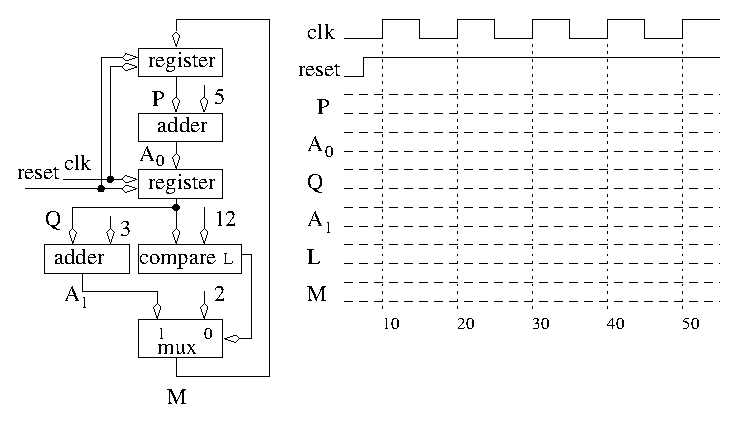
\includegraphics{./Fig2/BBBtiming2}

\item {\bf (2 pt.)}What is the value of $P$ at time 15?

\begin{tabular}{p{0.6in} p{0.6in} p{0.6in} p{0.6in} l}
a) 0 & b) 2 & c) 3 & d) 5 & e) 8
\end{tabular}

\item {\bf (2 pt.)}What is the value of $A_0$ at time 25?

\begin{tabular}{p{0.6in} p{0.6in} p{0.6in} p{0.6in} l}
a) 7 & b) 8 & c) 11 & d) 13 & e) 16
\end{tabular}

\item {\bf (2 pt.)}What is the value of $Q$ at time 35?

\begin{tabular}{p{0.6in} p{0.6in} p{0.6in} p{0.6in} l}
a) 7 & b) 8 & c) 11 & d) 13 & e) 16
\end{tabular}

\item {\bf (2 pt.)}What is the value of $A_1$ at time 45?

\begin{tabular}{p{0.6in} p{0.6in} p{0.6in} p{0.6in} l}
a) 8 & b) 10 & c) 13 & d) 16 & e) 19
\end{tabular}

\item {\bf (2 pt.)}What is the value of $M$ at time 55?

\begin{tabular}{p{0.6in} p{0.6in} p{0.6in} p{0.6in} l}
a) 2 & b) 8 & c) 10 & d) 11 & e) 12
\end{tabular}

\end{enumerate}
\end{document}
